\documentclass{article}

\begin{document}

\section{Partikelschwarmoptimierung}
Die Partikelschwarmoptimierung/particle swarm optimization (PSO) wurde zuerst von Dr. Kennedy und Dr. Eberhart in 1995 vorgestellt.
 Sie ist inspiriert vom Verhalten von Vogelschwärmen und Fischschulen. Jeder Teil wird als Partikel bezeichnet, die Gesamtheit als Schwarm.
\\ Die Partikel werden gleichverteilt über dem Suchbereich verteilt. Sie erhalten eine zufällige Startgeschwindigkeit. 
Der Suchraum hat \textbf{D} Dimensionen und \textbf{N} ist die Menge an Partikeln. Nun hat das \textbf{i}-te Partikel die Position X\textsubscript{i}=(x\textsubscript{i1},x\textsubscript{i2},x\textsubscript{i3},... ...,x\textsubscript{iD})
  und die Geschwindigkeit V\textsubscript{i}(v\textsubscript{i1},v\textsubscript{i2},v\textsubscript{i3},... ...,v\textsubscript{iD}). Außerdem speichert jedes Partikel seine beste Position P\textsubscript{ibest} und erhält die insgesamt beste Position P\textsubscript{gbest}. 
\\
Jedes Partikel updated seine Position nach den folgenden Gleichungen:\\
V\textsubscript{i}\textsuperscript{K+1}=wV\textsubscript{i}\textsuperscript{K}+c\textsubscript{1}r\textsubscript{1}(P\textsubscript{ibest}-X\textsubscript{i}\textsuperscript{K})+c\textsubscript{2}r\textsubscript{2}(P\textsubscript{gbest}-X\textsubscript{i}\textsuperscript{K})\\
$X_i^{K+1}=X_i^K+V_i^{K+1}$
\begin{itemize}

  \item k: Nummer der Iteration
  \item i: Nummer des Partikels
  \item w: Startgewicht, gibt an wie stark/schwach sich die Geschwinidgkeit pro Iteration verändert, um Divergenz zu vermeiden sollte es  kleiner als 1 gewählt werden
  \item c1,c2: kognitives und soziales Gewicht, positive Konstanten

\end{itemize}
Schritte der gründsätzlichen Durchführung der Partikelschwarmoptimierung:
\begin{enumerate}
  \item Initialisierung: Die Partikel werden gleichverteilt initialisiert und erhalten eine Startgeschwindigkeit
  \item Evaluierung: Die Partikel werden nach einer Fitnessevaluierung ausgewertet 
  \item Update P: Der so gewonnene Fitnesswert wird dem bisher besten Fitnesswert des Partikels verglichen, ist er besser wird $P_{ibest}=P_i$. Ist dieser Wert auch besser als $P_{gbest}$ so ersetzt $P_i P_{gbest}$
  \item Update Partikel: Die Position und Geschwindigkeit werden nach den obigen Formeln verändert.
  \item Wiederholung: Schritt 2 bis 4 werden nun bis Erreichen des Abbruchkriteriums wiederholt
\end{enumerate}\\

Hier gibt es nun noch verschieden Einflüsse auf die Umsetzung der Partikelschwarmoptimierung.
Das Abbruchkriterium kann unterschiedlich gewählt werden. Standardmäßig werden hier entweder die Anzahl der Iterationen im Vorhinein festgelegt oder der Algorithmus endet nach einer zu geringen Änderung nach mehreren Iterationen. 
Um die Konvergenz zu beschleunigen kann der $P_{ibest}$-Wert anstatt des persönlich besten Wertes den besten Wert eines bestimmten Umfelds speichern.
Der Wahl der Fitnessevaluierung muss hier ein großer Wert zukommen. Eine gut gewählte Fitnessfunktion kann die Konvergenz stark beschleunigen und somit den benötigten Rechenaufwand minimieren.\\
PSO teilt viele Merkmale mit genetischen Algorithmen. Beide basieren auf einer zufälligen Initialisierung ihrer Agenten und entwickeln diese Anhand einer Fitnessevaluierung weiter. Allerdings erfolgt der Informationsaustausch grundlegend unterschiedlich. Während bei einem genetischen Algorithmus alle Agenten untereinander Informationen austauschen, erfolgt dies bei einer PSO nur in eine Richtung, vom besten Partikel zu allen anderen.\\


\begin{figure}
  \centering
  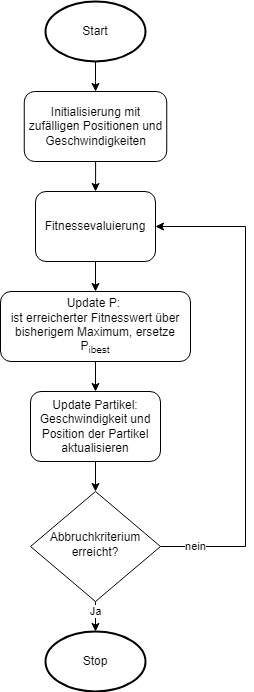
\includegraphics[scale=0.75]{Flow_PSO.png}
  \caption{Flussdiagramm von PSO}
  \label{fig:Figure_PSO}
\end{figure}


\section{Ameisen Algorithmen}
Ameisenalgorithmuen sind von der Futtersuche der Ameisen abgeleitet. Jede Ameise scheidet auf ihrem Weg Pheromone aus, welche mit der Zeit verdunsten. 
Folgende Ameisen wählen wahrscheinlicher einen Weg mit größerer Pheromonkonzentration. 
Existieren nun zwei unterschiedlich lange Wege mit gleicher Pheromonkonzentration, entscheiden sich etwa gleich viele Ameisen für beide Wege. 
Da die Ameisen auf dem kürzeren Weg in gleicher Zeit allerdings öfter laufen, steigt hier die Konzentration schneller als auf dem längeren Weg. 
Infolgedessen laufen immer mehr Ameisen den kürzeren Weg und es bildet sich eine Ameisenstraße.\\

Es gibt viele verschiedene Umsetzungen der Ameisenalgorithmen. Der erste Ansatz wurde von Marco Dorigo 1991 vorgestellt\cite{Dorigo1991AntSA} und 1996 nochmal verbessert\cite{484436}.
Sein Ansatz namens \emph{Ant System} lieferte Grundlagen welche er 1997 in einem neuen System namens \emph{Ant Colony System} weiter verbesserte\cite{585892}.\\
Schließlich veröffentlichte er in 2006 die \emph{Ant Colony Optimization (ACO)} welche im folgenden vorgestellt wird\cite{4129846} \\

Jede Ameise bewegt sich von Punkt x zu Punkt y mit folgender Wahrscheinlichkeit:\\
\large$p_{xy}^k=\frac{(T_{xy}^a)(n_{xy}^b)}{\Sigma(T_{xy}^a)(n_{xy}^b) }$

\begin{itemize}
  \item $T_x_y$: Menge an Pheromonen auf dem Übergang von x nach y 
  \item a: Gewicht des Einflusses von $T_x_y$
  \item $n_x_y$: Maß wie wünschenswert dieser Übergang ist, wird häufig aus Abstand zum Ziel berechnet
  \item b: Gewicht des Einflusses von $n_x_y$
\end{itemize}

Nun bewegt sich jeder Agent nach der von ihm berechneten Wahrscheinlichkeit, bis er den Zielzustand erreicht. Dann werden die Pheromone folgendermaßen aktualisiert:\\
$T_x_y^k=(1-p)T_x_y^k+\Delta T_x_y^k$
\begin{itemize}
  \item p: Pheromonverdunstung
  \item \delta $T_x_y$: in diesem Schritt ausgeschüttete Pheromone
\end{itemize}
Schritte der grundsätzlichen Durchführung von ACO:
\begin{enumerate}
  \item Initialisierung: Die Übergänge zwischen Start und Ziel bekommen einen Wert für n zugewiesen
  \item Jede Einheit bewegt sich einen Schritt übereinstimmend mit der berechneten Wahrscheinlichkeit.  Wiederholen, bis das Ziel erreicht ist
  \item Die Länge der Pfade messen und Pheromonkonzentration aktualisieren
  \item Die Länge aller Pfade mit dem bisherigen besten Pfad vergleichen, den besten Pfad speichern
  \item Wiederholung: Schritt 2-4 wiederholen bis Abbruchkriterium erreicht ist
\end{enumerate}

\begin{figure}
  \centering
  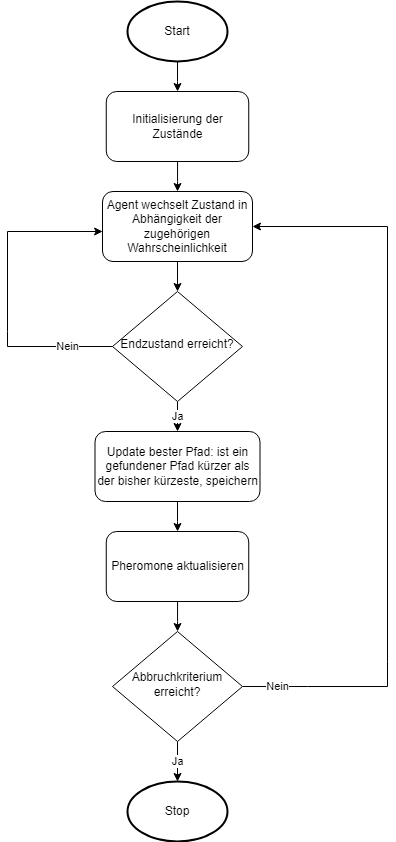
\includegraphics[scale=0.75]{Flow_ACO.png}
  \caption{Flussdiagramm von ACO}
  \label{fig:Figure_ACO}
\end{figure}

\section{Bienen Algorithmen}
Der Bienen Algorithmus ist von der Futtersuche der Bienen abgeleitet. Ein kleiner Teil des Bienenschwarms fungiert als Kundschafter für die Kolonie.
Sie sind konstant zufällig auf der Futtersuche. Finden sie eine Futterquelle analysieren sie deren Effektivität und kehren zum Bienenstock zurück. Die Effektivität hängt von Faktoren wie der Menge, Entfernung und Zuckergehalt ab.\cite{PHAM2006454}
Die Bienen, die eine effektive Futterquelle gefunden haben, führen nun einen sogenannten \emph{waggle dance} auf dem \emph{dance floor} aus \cite{Seeley+1995}. Damit gibt sie die Wegbeschreibung zur Futterquelle weiter.
Unbeschäftigte Arbeiterbienen schauen auf dem dance floor nach Wegbeschreibungen. Umso effektiver die Futterquelle, umso länger der Tanz, daher werden auch mehr Arbeiterbienen diese ausnutzen.\cite{KARABOGA2009108}\\

Im Artificial Bee Colony (ABC) Algorithmus gibt es drei Gruppen an Bienen:
\begin{enumerate}
  \item Kundschafter (Scout) Bienen: Sie fliegen zufällig auf der Futtersuche umher
  \item Betrachter Bienen: Sie stehen am dance floor und beobachten die Tänze. Sie suchen sich den besten aus und werden nun zu beschäftigten Bienen
  \item Beschäftigte Bienen: Sie fliegen zu der von ihr gewählten Futterquelle. Nachdem sie zurückgekehrt sind kommunizieren sie ihre Informationen auf dem dance floor weiter
\end{enumerate} 

Die Position einer Futterquelle repräsentiert  

\end{document}
